\documentclass[12pt]{article}
\usepackage[]{fullpage}
%\usepackage{a4wide}
\usepackage[]{graphics}
\usepackage{natbib}
\usepackage{setspace} 
\usepackage{url}
\usepackage{amsmath}
\usepackage{mathtools}
\renewcommand{\thesubsubsection}{\thesubsection.\alph{subsubsection}}

\title{Supervised and Unsupervised Learning on Lending Club Data}
\author{Muhammad Waqar Ayub Khan, UEA ID. 100334069}

\begin{document}

\maketitle

\begin{abstract}
	
\onehalfspacing

Classification and clustering are difficult tasks that can be used to predict results from various datasets. These are the tasks that make up the majority of data science work. On the lending club dataset, this study uses various KDD actions for classification and clustering, which enable the related institute to identifying whether a loan is potentially a bad loan or a good loan. To obtain reliable results, various machine learning algorithms for classification and clustering were applied to the dataset.

\end{abstract}
\doublespacing

\section{Introduction}
This report has two task, first task is to use lending club dataset and predict the loan status of the accounts, as we already know the loan status so this can be done by using different classification algorithms and then we can find the accuracy of our predictions by comparing the predicted results with the actual loan status. Second task is to use clustering algorithms to divide the data points into number of groups, each group represents the similar type of data points in our case loan status. Both tasks consists on Knowledge Discovery of Databases (KDD) steps, each step of KDD has a separate action on dataset which helps in getting more accurate results. In this study various techniques was used on dataset before making predictions such as removing abnormal data points known as Outliers, dealing with missing values, data balancing, dimensionality reduction which are the part of KDD process. Classification and clustering both involves these steps for accurate predictions, these steps are known as Cleaning and Pre-processing of a data. After getting cleaned and pre-processed data, for classification various algorithms were applied to get predictions and similarly for clustering predictions different clustering algorithms were applied to get accurate clusters. Overall both classification and clustering involve cleaning, pre-processing, modeling, evaluation, each step for both clustering and classification will be discussed in this report.

\section{Data / Feature Summary} 
Lending club data contains 108 different columns and have 77159 different loan account records. Out of 108 there 17 columns have more than 60 percent null values, having more much null values might lead to bad prediction so these features were dropped from the dataset and new dataset was created which has 91 columns or features with same number of rows. Figure \ref{fig:MissingValues} shows the feature having missing values greater than 60 percent.
\begin{figure}[h!]
	\centering
	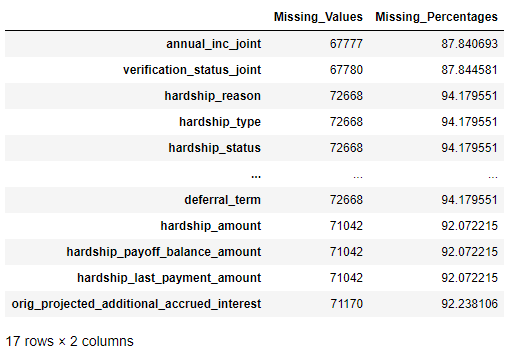
\includegraphics{MissingValues.png}
	\caption{Features having more than 6 percent missing values}
	\label{fig:MissingValues}
\end{figure}
After dropping these features we have a data with 91 features out of 91 14 features are categorical, which are shown in table \ref{table:1}.
\begin{table}[h!]
	\centering
	\begin{tabular}{ |p{3cm}|p{3cm}|p{3cm}|  }
		\hline
		\multicolumn{2}{|c|}{Categorical Features} \\

		\hline
		$emp\_title$ & 28185 \\
		$home\_ownership$ & 5 \\
		$loan\_status$ & 7 \\
		$int\_rate$ & 129 \\
		$term$ & 2 \\
		$grade$ & 7 \\
		$earliest\_cr\_line$ & 622 \\
		$issue\_d$ & 16 \\
		$last\_pymnt\_d	$ & 28 \\
		$next\_pymnt\_d	$ & 9 \\
		$verification\_status$ & 3 \\
		$pymnt\_plan$ & 1 \\
		$purpose$ & 13 \\
		$revol\_util$ & 1074 \\
		\hline
	\end{tabular}
	\caption{List of Categorical Features with unique values}
	\label{table:1}
\end{table}
 Features named such as id, $emp\_title$ will be dropped because these two has too many unique values, $pymnt\_plan$ will also be dropped because it has only one unique value. $int\_rate$ and $revol\_util$ will be converted to numeric after removing $\%$ symbol from the last similarly $term$ will be converted to numeric after removing $months$ from last. There are some dates columns or features in the data we can use these dates and can convert those dates into some useful information like missing term or remaining term. Figure \ref{fig:dates} shows the features which have been transformed from the dates columns. $loan\_status$ is a target feature which will be separated from the other columns or features. The remaining categorical features or columns will now be encoded into the numeric so that these features can be dealt by modeling algorithms. These are encoded before the train-test split because encoding before split reduce the computation and does not expose the test data to the training model. After feature engineering, encoding the new data has only one categorical feature which is $loan\_status$ and it will be remove from data as it is target feature and new data has now 85 columns or features and 77159 records.

\begin{figure}[h!]
	\centering
	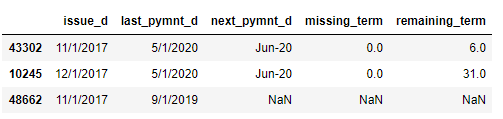
\includegraphics{dates.png}
	\caption{Transformation of Dates Columns}
	\label{fig:dates}
\end{figure}

\section{Classification}
In classification the task is to identify the status of the loan whether a loan is a good loan or a bad loan. In the actual data we have seven different status of the loan e-g $fully\_paid$, $Current$, $charged\_off$, $late\_15\_30\_days$, $late\_30\_120\_days$, , $grace\_period$, , $default$. Status like $charged\_off$, $late\_15\_30\_days$, $late\_30\_120\_days$, , $grace\_period$, , $default$ represent the bad loan so these statuses converted into the 1 class which is named as $bad\_loan$. Now our classification problem is converted into three class classification problem $fully\_paid$ which is a good loan, $bad\_loan$ which represents the loans which are bad investments by thee banks and $Current$ loans which are still under observations. Figure \ref{fig:classes} shows the statuses of the loans in the dataset.
\begin{figure}[h!]
	\centering
	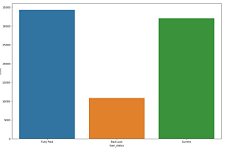
\includegraphics{classes.png}
	\caption{Loan Status Classes}
	\label{fig:classes}
\end{figure}
The working flow for the classification is well explained in the figure \ref{fig:c_flow}.
\begin{figure}[h!]
	\centering
	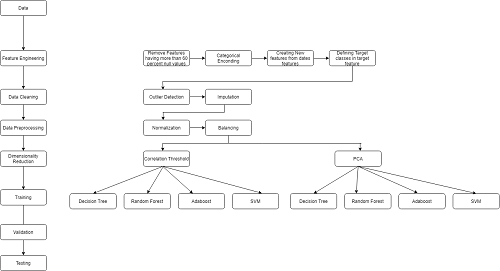
\includegraphics[width=\textwidth]{c_flow.png}
	\caption{Classification Flow}
	\label{fig:c_flow}
\end{figure}
In classification section, train-test split is done just after the feature engineering where we create some new features like $missing\_term$, $remaining\_duration$ by using dates features in the dataset. Removing test set before the cleaning and pre-processing prevents data leakage, test data remains unexposed to the training model while doing cleaning and pre processing of the training data, cleaning and pre processing on test set is done separately. The steps involve in each phase of the classification is describe below.
\subsection{Data Cleaning}
Data cleaning is used to eliminate noise, inconsistencies, and inaccuracies from training data. This should allow for the development of a viable classification model using a more comprehensive and representative data set. Unclean data can sometimes influence the classification accuracy of a model in most classification methods. Data cleaning involves outlier handling and imputation of the missing values.
\subsubsection{Outlier Detection}

In a dataset, an outlier is a value that is abnormally far off from other values. In some ways, this definition delegated the decision of what is abnormal to the analyst. Outliers can be detected or dealt with using a variety of methods. Outlier detection approaches must be chosen based on the dataset. If a dataset has too many outliers, we must place those observations under distributions to see what they represent. Another method is to use algorithms to detect outliers and delete them from the dataset. To make things simpler in this problem Isoloation forest algorithm is used which is outlier detection algorithm to detect abnormal points and than those points were removed from the dataset to make dataset cleaner. The result of isolation forest is that there are more than 6000 outliers in the dataset which should be remove from the dataset. To make things easier in our case, the Isolation forest technique is utilised, which is an outlier identification technique that detects anomalous points and then removes those points from the dataset to clean it up. The  result of the isolation forest is that there are more than 6000 outliers in the dataset that need to be removed.

\subsubsection{Imputation}
Imputation is another important step in data cleaning because if there are missing values in the dataset than if we try to create a model with missing values, most machine learning algorithms gives an error. As a result, you'll need to pick one of the imputation tactics. There are many techniques for the imputation of missing values in the dataset such as dropping the rows, imputing with nearest values, imputing with up and down values or imputing with mean value. For simplicity in our case Mean-imputation is used, because imputing with mean preserves the mean of that particular feature, the estimate of the mean remains unbiased. There are benefits and disadvantages of mean imputation that are not in the scope of this project.

\subsection{Data Transformation}
Data transformation is the process of taking raw data, normalising it, balancing it, and transforming it into data that can be put together for analysis. Although dimensionality reduction is a part of data transformation, it is treated as a separate phase in this report since a comparison research was undertaken to obtain more accurate findings with dimensionality reduction. Normalization and balancing of the data are the two steps which were performed in transformation phase which are describe below.
\subsubsection{Normalization}
Normalization is a data transformation method that is regularly utilized in machine learning. Normalization is the way toward changing over the upsides of numeric columns in a dataset to a comparable scale without influencing the ranges of values. Neural Network also uses normalization to make data normalize which reduces computational time. Many machine learning algorithms, such as support vector machines and k means, are sensitive to normalization, although many others algorithm may function without it. Also because dimensionality reduction techniques like Principle Component Analysis (PCA) are sensitive to normalization, we must do normalization before dimensionality reduction.

\subsubsection{Data Balancing}
Imbalanced data occurs when the amount of observations for all of the classes in a classification dataset is not equal. Many machine learning classifiers struggle with unbalanced training datasets because they are sensitive to the ratios of various classes. As a result, these algorithms prefer the class with the highest set of observations, which might lead to inaccurate results. This can be especially problematic when we are looking for the rare class identification since many algorithms are unable to find sufficient data for learning. We can delete entries from the majority class to balance the data, but this may result in the loss of some crucial information; another option is to add duplicate values, which is also inefficient. For our study SMOTE technique is used for balancing the data, SMOTE creates new records rather than duplicating the records from the dataset which is very good for highly imbalanced data.


\subsection{Dimensionality Reduction}


\subsection{Training}

\subsection{Validation}

\subsection{Testing}
\section{Clustering}


\section{Conclusion}


\singlespacing

\bibliographystyle{agsm}
\bibliography{document}

\end{document}




